\subsection{Domains of Protection}\label{subsec:Domains_of_Protection}
A computer system is a collection of \nameref{def:Process}es and objects.
Objects refer to:
\begin{itemize}[noitemsep]
\item Hardware Objects
  \begin{itemize}[noitemsep]
  \item CPU
  \item Memory Segments
  \item Printers
  \item Disks
  \item Tape Drives
  \end{itemize}
\item Software Objects
  \begin{itemize}[noitemsep]
  \item Files
  \item Programs
  \item Semaphores
  \end{itemize}
\end{itemize}

Each object has a unique name that differentiates it from all other objects in the system, and each can be accessed only through well-defined and meaningful operations.
The operations that are possible depends on the object in question.
For example, on a CPU, we can perform executions, memory can be read from and written to, etc.

A \nameref{def:Process} should be allowed to access only those resources for which it has authorization.
Furthermore, at any time, a process should be able to access only those resources that it currently requires to complete its task.
This second requirement, is commonly referred to as the \nameref{def:Need_To_Know_Principle}.

\begin{definition}[Need-to-Know Principle]\label{def:Need_To_Know_Principle}
  The \emph{Need-to-Know principle} states that a \nameref{def:Process} should be able to access \textbf{only} those resources that it currently requires to complete its \textbf{current} task.

  This is useful in limiting the amount of damage a faulty process can cause in the system.
\end{definition}

\subsection{Domain Structure}\label{subsubsec:Domain_Structure}
A \nameref{def:Process} operates within a \nameref{def:Protection_Domain}.

\begin{definition}[Protection Domain]\label{def:Protection_Domain}
  A \emph{protection domain} specifies the resources that a \nameref{def:Process} may access.
  Each domain defines a set of objects and \nameref{def:Access_Right}s.
  A domain is a collection of access rights, each of which is an ordered pair

  \begin{equation}\label{eq:Protection_Domain}
    \langle \text{object-name}, \text{rights-set} \rangle
  \end{equation}
\end{definition}

A \nameref{def:Protection_Domain} can be defined in many ways.
\begin{itemize}[noitemsep]
\item Each user may be a domain. In this case, the set of objects that
  can be accessed depends on the identity of the user. Domain
  switching occurs when the user is changed —generally when one user
  logs out and another user logs in.
\item Each process may be a domain.
  In this case, the set of objects that can be accessed depends on the
  identity of the process. Domain switching occurs when one process
  sends a message to another process and then waits for a response.
\item Each procedure may be a domain. In this case, the set of objects
  that can be accessed corresponds to the local variables defined
  within the procedure. Domain switching occurs when a procedure call
  is made.
\end{itemize}

\begin{definition}[Access Right]\label{def:Access_Right}
  The ability to execute an operation on an object is an \emph{access right}.
\end{definition}

\nameref{def:Protection_Domain}s may share \nameref{def:Access_Right}s.
For example, if we have three domains: $D_{1}$, $D_{2}$, and $D_{3}$ an an access right $\langle O_{4}, \text{print} \rangle$ that is shared by $D_{2}$ and $D_{3}$, a process executing in either of these domains can print object $O_{4}$.

The association between a \nameref{def:Process} and a \nameref{def:Protection_Domain} may be either \textbf{static}, if the set of resources available to the process is fixed throughout the process’s lifetime, or \textbf{dynamic}.

\subsubsection{Static Domain Structure}\label{subsubsec:Static_Domain_Structure}
A static association between \nameref{def:Process}es and \nameref{def:Protection_Domain}s is possible, but it is not a very flexible system, and makes it difficult to adhere to the need-to-know principle.
To counter this, a mechanism must be available to change the content of a domain.

This mechanism is needed because a \nameref{def:Process} may execute in two different phases and may, for example, need read access in one phase and write access in another.
If the \nameref{def:Protection_Domain} is static, the domain must be defined to include \textbf{both} read and write access throughout the process's execution.

However, this arrangement provides more rights than are needed in each of the two phases, since we have read access in the phase where we need only write access, and vice versa.

\subsubsection{Dynamic Domain Structure}\label{subsubsec:Dynamic_Domain_Structure}
A dynamic association between \nameref{def:Process}es and \nameref{def:Protection_Domain}s relies on a mechanism to allow \nameref{def:Domain_Switching}.

\begin{definition}[Domain Switching]\label{def:Domain_Switching}
  \emph{Domain switching} is a tool that enables a \nameref{def:Process} to switch from one \nameref{def:Protection_Domain} to another.
  We may also allow the content of a domain to be changed.
\end{definition}

If we cannot change the content of a domain, we can provide the same effect by creating a new domain with the changed content and switching to that new domain when we want to change the domain content.

\subsubsection{\textsc{unix}-Style Protection Domains and Schemes}\label{subsubsec:UNIX_Protections}
In the \textsc{unix} operating system, a domain is associated with the \nameref{def:User}.
Switching the domain corresponds to changing the user identification.

This change is accomplished through the \nameref{def:File_System}.
Each file contains a lot of metadata regarding the attributes of the file, including who owns the file and to which domain (\nameref{def:User}) that files belongs to.
The first one is the file's owner identification (\texttt{userID}); the second is the \texttt{setuid} bit (the domain bit).

When the \texttt{setuid} bit is on, and a \nameref{def:User} executes that file, the process that is created has its \texttt{userID} set to the owner of the file.
When the \texttt{setuid} bit is off, the \texttt{userID} does not change.
For example, when a user $A$ (that is, a user with \texttt{userID} = $A$) starts executing a file owned by $B$, whose associated domain bit is off, the \texttt{userID} of the process is set to $A$.
When the \texttt{setuid} bit is on, the \texttt{userID} is set to that of the owner of the file: $B$.
When the process exits, this temporary \texttt{userID} change ends.

Other methods are used to change domains in operating systems in which \texttt{userID}s are used for domain definition.
This mechanism is used when an otherwise privileged facility needs to be made available to the general user population.
For instance, it might be desirable to allow users to access a network without letting them write their own networking programs.
On a \textsc{unix} system, the \texttt{setuid} bit on a networking program would be set, causing the \texttt{userID} to change to another \texttt{userID} that is capable of using the network when the program is run.
The \texttt{userID} would change to that of a user with network access privilege (such as \texttt{root}).
One problem with this method is that if a user manages to create a file with \texttt{userID} root and with its \texttt{setuid} bit on, that user can become root and do anything and everything on the system.

An alternative to this method used in some other \nameref{def:Operating_System}s is to place privileged programs in a special \nameref{def:Directory}.
The operating system is designed to change the \texttt{userID} of any program run from this directory.
This eliminates the security problem of when intruders create programs to manipulate the \texttt{setuid} feature and hide the programs in the system for later use.
This method is less flexible than that used in \textsc{unix}, however.

Even more restrictive, and thus more protective, are systems that simply do not allow a change of \texttt{userID}.
In these \nameref{def:Operating_System}s, special techniques must be used to allow users access to privileged facilities.
One method, for instance, is to use a \nameref{def:Daemon} process that is started at boot and runs as a special \texttt{userID}.
Regular \nameref{def:User}s then run a separate program, which sends requests to this process whenever they need to use the facility.

In any of these systems, great care must be taken in writing privileged programs.
Any oversight can result in a total lack of protection on the system.

\subsubsection{\textsc{multics}-Style Protection Domains and Schemes}\label{subsubsec:MULTICS_Protections}
In the \textsc{multics} system, the \nameref{def:Protection_Domain}s are organized hierarchically into a ring structure.
Each ring corresponds to a single domain, see \Cref{fig:MULTICS_Rings} for a visualization.

\begin{figure}[h!tbp]
  \centering
  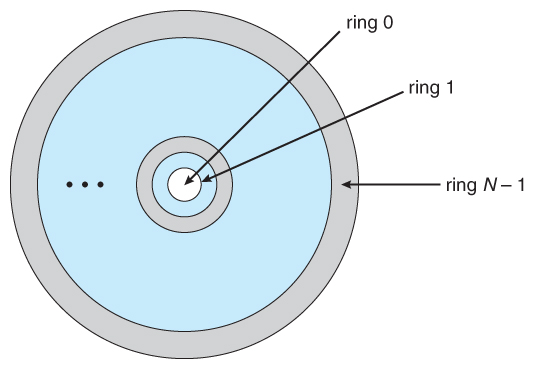
\includegraphics[scale=1.00]{./Drawings/EDAF35-Operating_Systems/MULTICS_Rings.jpg}
  \caption{\textsc{multics} Rings}
  \label{fig:MULTICS_Rings}
\end{figure}

The rings are numbered from 0 to $N-1$.
Let $D_{i}$ and $D_{j}$ be any two domain rings.
If $j < i$, then $D_{i}$ is a subset of $D_{j}$, meaning a \nameref{def:Process} executing in domain $D_{j}$ has more privileges than a process executing in domain $D_{i}$.
A process executing in domain $D_{0}$ has the most privileges.
\begin{remark*}
  If only two rings exist, this scheme is equivalent to the monitor–user mode of execution, where monitor-/\nameref{def:Kernel}-mode corresponds to $D_{0}$ and \nameref{def:User}-mode corresponds to $D_{1}$.
\end{remark*}

\textsc{multics} has a segmented address space; each segment is a file, and each segment is associated with one of the rings.
A segment description includes an entry that identifies the ring number that it is associated with.
In addition, it includes three access bits to control reading, writing, and execution.
The association between segments and rings is a policy decision.

A \texttt{current-ring-number} counter is associated with each \nameref{def:Process}, identifying the ring in which the process is executing currently.
Given 3 ring domains $i$, $j$, and $k$, where $j < i$ and $k \geq i$, and the process is executing in ring $i$, the process cannot access a memory segment associated with ring $j$, but \emph{can} access a segment associated with ring $k$.
In terms of \Cref{fig:MULTICS_Rings}, this means a process can always move outwards from the center to access memory, but never inwards.
A process in ring $i$ accessing ring $k$'s memory segment when $i \geq k$ is restricted according to the access bits associated with that segment.

Domain switching in \textsc{multics} occurs when a process crosses from one ring to another by calling a procedure in a different ring.
This switch must be done in a controlled manner; otherwise, a process could start executing in ring $0$, and no protection would be provided.
To allow controlled domain switching, the ring field of the segment also includes:
\begin{itemize}[noitemsep]
\item \textbf{Access bracket}.
  A pair of integers, $\langle b_{1}, b_{2} \rangle$, where $b_{1} \leq b_{2}$.
\item \textbf{Limit}.
  An integer $b_{3}$ such that $b_{3} > b_{2}$.
\item \textbf{List of gates}.
  Identifies the entry points (or gates) at which the segments may be called.
\end{itemize}

If a process executing in ring $i$ calls a procedure (or segment) with access bracket $\langle b_{1}, b_{2} \rangle$, then the call is allowed if $b_{1} \leq i \leq b_{2}$, and the current ring number of the process remains $i$.
Otherwise, a \nameref{def:Trap} to the \nameref{def:Operating_System} occurs, and the situation is handled.
\begin{itemize}[noitemsep]
\item If $i < b_{1}$, then the call is allowed to occur, because we have a transfer to a ring with fewer privileges.
  If parameters are passed that refer to segments in a lower ring (that is, segments not accessible to the called procedure), then these segments must be copied into an area that can be accessed by the called procedure.
\item If $i > b_{2}$, then the call is allowed to occur only if $b_{3}$ is greater than or equal to $i$ and the call has been directed to one of the designated entry points in the list of gates.
  This scheme allows processes with limited access rights to call procedures in lower rings that have more access rights, but only in a carefully controlled manner.
\end{itemize}

The main disadvantage of the ring structure is that it does not allow us to enforce the \nameref{def:Need_To_Know_Principle}.
In particular, if an object must be accessible in domain $D_{j}$ but not accessible in domain $D_{i}$, then we must have $j < i$.
But this requirement means that \textbf{every} segment accessible in $D_{i}$ is also accessible in $D_{j}$.

The \textsc{multics} protection system is generally more complex and less efficient than are those used in current operating systems.

%%% Local Variables:
%%% mode: latex
%%% TeX-master: "../../EDAF35-Operating_Systems-Reference_Sheet"
%%% End:
